\documentclass[conference]{IEEEtran}
\IEEEoverridecommandlockouts
% The preceding line is only needed to identify funding in the first footnote. If that is unneeded, please comment it out.
\usepackage{cite}
\usepackage{amsmath,amssymb,amsfonts}
\usepackage{algorithmic}
\usepackage{graphicx}
\usepackage{textcomp}
\usepackage{xcolor}
\usepackage{hyperref}
\usepackage{float}
\def\BibTeX{{\rm B\kern-.05em{\sc i\kern-.025em b}\kern-.08em
    T\kern-.1667em\lower.7ex\hbox{E}\kern-.125emX}}
\begin{document}

\title{Unblock Me}

\author{\IEEEauthorblockN{Guilherme Silva (201603647)}
\IEEEauthorblockA{\textit{IART} \\
\textit{FEUP}\\
Porto, Portugal \\
up201603647@fe.up.pt}
\and
\IEEEauthorblockN{Miguel Duarte (201606298)}
\IEEEauthorblockA{\textit{IART} \\
\textit{FEUP}\\
Porto, Portugal \\
up201606298@fe.up.pt}
\and
\IEEEauthorblockN{Rui Alves (201606746)}
\IEEEauthorblockA{\textit{IART} \\
\textit{FEUP}\\
Porto, Portugal \\
up201606746@fe.up.pt}
}

\maketitle

% TODO
\begin{itemize}
    \item Update abstract
    \item Update introduction
    \item Fix Operators - Move several cells with cost 1 instead of just 1
    \item Game implementation section
    \item search algorithms section
    \item experiments and results section
    \item update conclusion
\end{itemize}


\begin{abstract}
The aim of this paper is to implement and compare Artificial Intelligence algorithms for solving the game \textit{Unblock Me}, in which rectangular pieces block the path of a red special piece. The objective of the game is for the special piece to reach the exit of the level, which is achieved by moving it and the other pieces.
The problem will be described and then formulated as a \textit{Search Problem}, together with some discussion on the reasoning behind some of the decisions taken during this process.
Several algorithms will be investigated, along with testing them against levels with varying difficulty and branching factors. Both the efficiency in reaching a solution and the cost of the calculated solution will be taken into account in the pursuit for the optimal \textit{Search Algorithm}.
\end{abstract}

\begin{IEEEkeywords}
Artificial Intelligence, Search Problems, Path-finding algorithms, Decision-making Heuristics, Graph Algorithms, Depth-First Search, Breadth-First Search, Uniform Cost Search, Iterative Deepening, Greedy Search, A*, Bi-Directional Search
\end{IEEEkeywords}

\section{Introduction}
The game that is the subject of study in this paper (\textit{Unblock Me}) will be approached with several different \textit{Search Algorithms}, implemented in \textit{Python}, in order to conclude what is the best approach for solving it using \textit{Artificial Intelligence Algorithms}.

Firstly, the game will be described in further detail, ensuring that all non-formal aspects of it are well documented. Secondly, it will be formulated as a \textit{Search Problem}, with the approach taken in doing so being illustrated in increased depth, providing reasoning for the decisions taken. Thirdly, a research on related work on this topic will be presented, giving some insight on the problem from other points of view.

Finally, a small section will cover the conclusions and future work, by expanding on the already developed tasks and elaborating on the planned approach.

\section{Problem Description}
\textit{Unblock Me} is a puzzle game that was released in 17-06-2009 by \textit{Kiragames}. It is an adapted version of \textit{Rush Hour}, a puzzle game invented by Nobuyuki Yoshigahara in the 1970s. Each level consists of a 6x6 board, surrounded with walls (except for the puzzle's exit) \cite{b1}.

\begin{figure}[H]
    \centerline{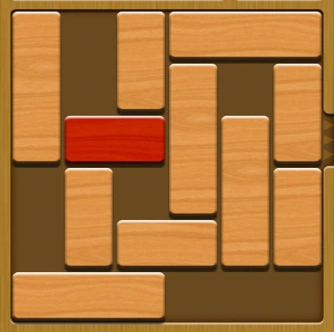
\includegraphics[width=100px]{img1.png}}
    \caption{Example of an \textit{Unblock Me} level}
\end{figure}

The game's objective is to move a special piece to the level's exit, by moving that and the other pieces with the least number of movements possible. Pieces are rectangles with a given orientation (vertical or horizontal) and constant length. Pieces can only move in the direction of their orientation into empty cells (they may not overlap).  

\begin{figure}[H]
    \centerline{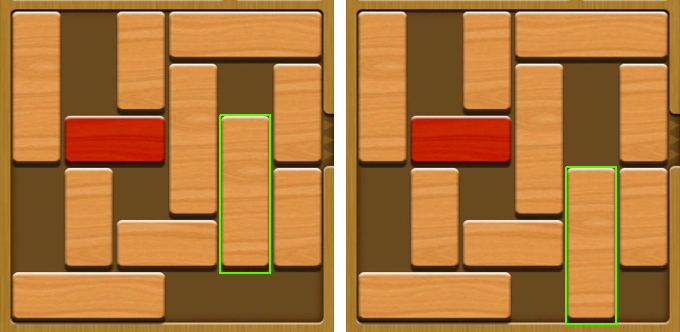
\includegraphics[width=200px]{img2.png}}
    \caption{Piece moving down one cell}
\end{figure}

Levels are fully surrounded by walls, except for the level's exit door that is alligned with the special piece and by which only the special piece can go through. The level is completed once the piece goes through the exit door.
 
\begin{figure}[H]
    \centerline{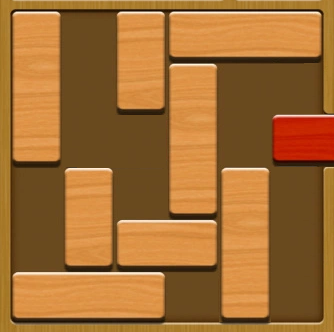
\includegraphics[width=100px]{img3.png}}
    \caption{Beating a level by going through the exit}
    \label{img:final_state}
\end{figure}

Some levels may even contain fixed blocks that can not be moved, representing obstacles.
 
\begin{figure}[H]
    \centerline{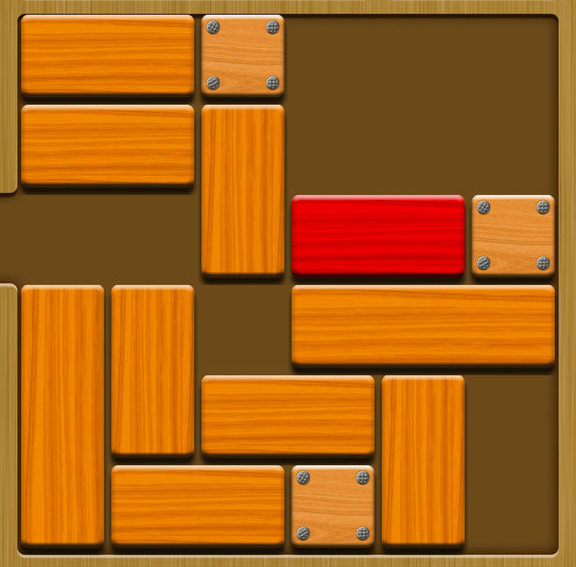
\includegraphics[width=100px]{img4.png}}
    \caption{Example of an \textit{Unblock Me} level containg fixed blocks}
\end{figure}

\section{Problem Formulation}
The game's solving process can be formulated as a search problem, in which the goal is to find the sequence of moves (state transitions) that take the special piece to the level's exit door - the problem's goal state. 

\subsection{Game State Representation} \label{subsec:gr}

\begin{itemize}
    \item List of pieces, where each piece contains the following information:
    \begin{itemize}
        \item Origin Square (top left piece corner, e.g. (0,0))
        \item Length (e.g. 4)
        \item Direction (H or V)
    \end{itemize}
    \item Reference to the special piece
    \item Matrix of booleans, where True means the cell is empty
\end{itemize}

This representation of the game state makes the generation of valid movements easier, due to the fact that to determine possible movements of a single piece, the other pieces do not need to be taken into account (assuming that all empty cells are known). Thus, to generate all possible branching options, the list of pieces needs to be iterated over, while checking if there are empty cells adjacent to the piece's extremities (these change with the piece's direction). This representation facilitates the execution of these tasks, making it less costly (important fact due to high number of operations of this kind):

\begin{itemize}
    \item Using a list of pieces makes it trivial to determine which of them can be moved in a given state;
    \item Using a matrix (of booleans, that state if a cell is occupied or not) makes it trivial to check if adjacent cells to the pieces extremities are empty;
    \item Finnaly, using a reference to the special piece allows accessing it in constant time, which will be useful to heuristic related operations and determine if the goal state (\autoref{subsec:gs}) is achieved.
\end{itemize}

\subsection{Initial State}
The initial state depends of the level in question, being represented by a game state as described in \autoref{subsec:gr}.

\subsection{Goal State} \label{subsec:gs}
The goal state consists of a piece configuration where the special piece reaches the level exit (\autoref{img:final_state}).

\subsection{Operators}
\begin{itemize}
    \item Move piece to the left:
    \begin{itemize}
        \item Pre-conditions:
        \begin{itemize}
            \item Piece with horizontal orientation
            \item Cell that is adjacent to the piece's left extremity must be empty
        \end{itemize}
        \item Results: The pieces position moves one cell to the left
        \item Cost: 1 movement
    \end{itemize}
    \item Move piece to the right:
    \begin{itemize}
        \item Pre-conditions:
        \begin{itemize}
            \item Piece with horizontal orientation
            \item Cell that is adjacent to the piece's right extremity must be empty
        \end{itemize}
        \item Results: The pieces position moves one cell to the right
        \item Cost: 1 movement
    \end{itemize}
    \item Move piece up:
        \begin{itemize}
        \item Pre-conditions:
        \begin{itemize}
            \item Piece with vertical orientation
            \item Cell that is adjacent to the piece's top extremity must be empty
        \end{itemize}
        \item Results: The pieces position moves one cell up
        \item Cost: 1 movement
    \end{itemize}
    \item Move piece down:
    \begin{itemize}
        \item Pre-conditions:
        \begin{itemize}
            \item Piece with vertical orientation
            \item Cell that is adjacent to the piece's bottom extremity must be empty
        \end{itemize}
        \item Results: The pieces position moves one cell down
        \item Cost: 1 movement
    \end{itemize}
\end{itemize}

\subsection{Path cost}
The solution's path cost that is to be minimized is equal to the number of movements made (number of state transitions).


\section{Related Work}
\textit{Unblock Me} is also widely known as \textit{Rush Hour}. In June 2018, Michael Fogleman (a Software Engineer at Formlabs) developed an artificial intelligence that solves the puzzle and created a database with over two million and a half different puzzles\cite{b2}. His solution is based in the usage of bitboards\cite{b3} (data structure that is often used by board games computer systems due to its short space usage and operations efficiency) for the game states representation. 

This game is also studied in the Computer Science MSc from the University of Princeton, namely in the course "Computer Science 402 - Artificial Intelligence". In this course, students implement multiple heuristics to solve the problem using the A* algorithm\cite{b4}. Rainhard Findling, a researcher in Aalto University in Finland, proposes a solution to this problem statement, by using a heuristic based on a vote system, where each piece that is blocking the way of the special piece to the level's exit votes on how they want to free the way (how many moves they have to perform) for the special piece\cite{b5}. 

Even though that the problem is not complex, the increasing of the board size quickly leads to a combinatorial explosion, being that a 6x6 board has over 27 billion possible states. Thus, it is not efficient to find a solution by exploring all the possible states, being a good heuristic for state exploration mandatory.

\section{Game Implementation}
aa

\section{Search Algorithms}
aa

\section{Experiments (Tests?) and Results}
aa

\section{Conclusions and Future Work}
As of yet, the problem has been completely formalized - it has been formally described, and formulated as a search problem (a Game State representation has been reached, the initial and goal states have been described and the operators and path cost have been stated).

The chosen programming language was Python, and a simple graphical interface has been implemented, in order to show the solutions of the different algorithms when they are implemented.

In order to study the best possible approach for solving \textit{Unblock Me} puzzles, the following algorithms will be the subject of various tests:
\begin{itemize}
    \item Breadth-First Search
    \item Depth-First Search
    \item Iterative Deepening
    \item Uniform Cost Search
    \item Greedy Search
    \item A*
    \item Bi-Directional Search (using Greedy Search)
    \item Bi-Directional Search (using A*)
\end{itemize}

For the informed search algorithms (Greedy and A*), several different heuristics will be experimented with, such as:

\begin{itemize}
    \item The number of pieces between the special piece and the level exit
    \item The number of cells (distance) between the special piece and the level exit
\end{itemize}

In order to evaluate the implemented algorithms, they will be assessed both in terms of the achieved solution's quality and in terms of the algorithm's performance. For the first metric, the main evaluation point will be the number of piece movements. For the latter, both the execution time and the number of evaluated states will be taken into account.

\begin{thebibliography}{00}
    
\bibitem{b1} "Unblock me FREE.". Google Play. February 28, 2019.\href{https://play.google.com/store/apps/details?id=com.kiragames.unblockmefree}{https://play.google.com/store/apps/details?id=com.kiragames.unblo\\ckmefree}.
\bibitem{b2} Fogleman, Michael. "Solving Rush Hour, the Puzzle.". July, 2018. \href{https://www.michaelfogleman.com/rush/}{https://www.michaelfogleman.com/rush/}.
\bibitem{b3} "Bitboard.". Wikipedia - The free Encyclopedia. December 6, 2018. \href{https://en.wikipedia.org/wiki/Bitboard}{https://en.wikipedia.org/wiki/Bitboard}.
\bibitem{b4} Littman, Michael. "Programming Assignment P1 - What A* Rush". Priceton. 2012. \href{https://www.cs.princeton.edu/courses/archive/fall12/cos402/assignments/programs/rushhour/}{https://www.cs.princeton.edu/courses/archive/fall12/cos402/assignments\\/programs/rushhour/}.
\bibitem{b5} Findling, Rainhard. "The RushHour Puzzle – an Artificial Intelligence Toy Problem.". April 4, 2012. \href{http://geekoverdose2.rssing.com/browser.php?indx=39804402\&item=1}{http://geekoverdose2.rssing.com/browser.php?indx=39804402\&item=1}.
\end{thebibliography}

\end{document}
